% !Mode:: "TeX:UTF-8"
% !TeX root = ../thesis.tex

\chapter{基于双目视觉的感知技术研究}
环境感知是两轮平衡车实现自动行驶的关键环节，其性能直接影响障碍物识别、距离估计与避障决策的可靠性。为提升车辆在实际场景中的环境理解能力，需要构建兼顾深度恢复与目标定位的感知方法。本章围绕双目视觉环境感知方法展开研究，面向模型轻量化与部署需求，研究兼顾精度与实时性的基于深度学习的立体匹配算法，以获取高质量视差图并恢复场景深度信息，为障碍物测距、空间定位及后续环境理解提供基础；研究基于深度学习的目标检测算法，并结合深度图实现障碍物目标的识别与空间定位，从而为后续导航与避障提供更加可靠的环境感知信息。

\section{基于深度学习的立体匹配技术研究}

立体匹配旨在通过双目图像对计算视差图，从而恢复场景的深度信息，是视觉感知中的关键技术之一。对于公园等半结构化场景，稳定的视差估计可为障碍物测距、空间定位和后续避障决策提供基础。传统方法在纹理丰富区域表现良好，但在遮挡、低纹理等复杂场景下易出现误匹配，且难以兼顾精度与实时性。近年来，基于深度学习的立体匹配方法在精度和鲁棒性方面取得显著进展，展现出更强的场景适应能力\cite{tosiSurveyDeepStereo2025,zhangReviewStereoMatching2024}。

\subsection{双目测距原理及相机标定}

在理想平行双目成像模型下，视差与深度呈反比关系，其几何关系如图\ref{理想双目模型}所示。设左右相机光轴平行、成像平面共面，双目基线沿水平方向布置，且图像已完成极线校正。记空间点$P$在左右像平面上的像素坐标分别为$p_l=[x_l,y_l]^T$和$p_r=[x_r,y_r]^T$，则对应点满足$y_l=y_r$，其水平视差为$d=x_l-x_r$。根据相似三角形关系，空间点深度$Z$与视差$d$之间满足式~\eqref{eq:ch3-geometry}：
\begin{equation}\label{eq:ch3-geometry}
Z=\frac{fB}{d}
\end{equation}
\begin{tabularx}{\textwidth}{@{}l@{\quad}r@{———}X@{}}
式中& $Z$ & 空间点到相机的深度值；\\
& $d$ & 左右图像对应点的水平视差；\\
& $f$ & 相机有效焦距；\\
& $B$ & 双目基线长度；\\
\end{tabularx}\vspace{3.15bp}

\begin{figure}[h]
  \centering
  \includesvg[width=0.45\textwidth]{figures/chapter03/理想双目模型}
  \caption{理想双目模型}
  \label{理想双目模型}
\end{figure}

实际双目系统受镜头畸变与安装误差影响，因此在利用式~\eqref{eq:ch3-geometry}进行测距前，需先完成双目标定、去畸变与立体校正。本文采用张正友标定方法，利用MATLAB的Stereo Camera Calibrator采集多组棋盘格图像进行双目标定，标定过程界面如图\ref{双目标定过程界面}所示。标定后可获得左右相机的内参矩阵$K_l,K_r$、畸变参数$D_l,D_r$以及双目系统的相对位姿$R,t$，为后续图像校正、极线约束建立和深度计算提供几何参数基础。

\begin{figure}[h]
  \centering
  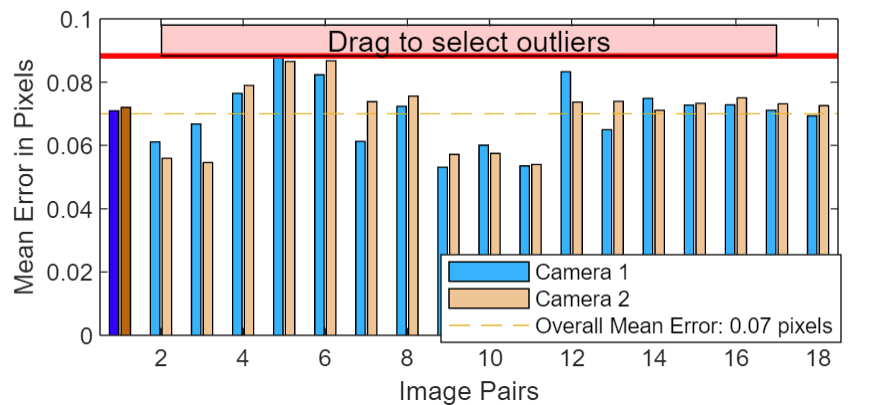
\includegraphics[width=0.48\textwidth]{figures/chapter03/双目相机标定结果A.png}
  \hfill
  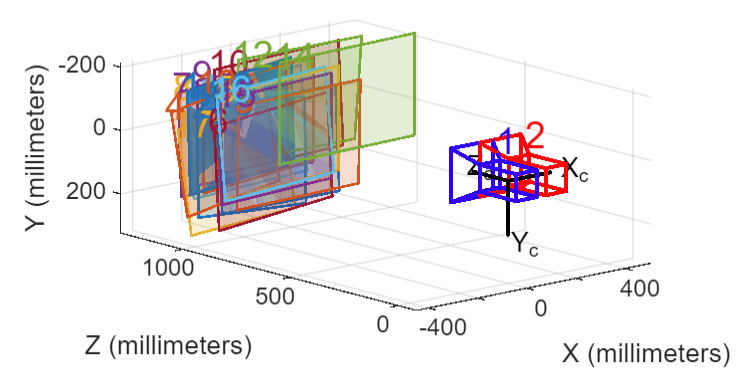
\includegraphics[width=0.48\textwidth]{figures/chapter03/双目相机标定结果B.png}
  \caption{双目标定过程界面}
  \label{双目标定过程界面}
\end{figure}

首先，对原始图像进行去畸变。设畸变像素点与去畸变像素点的齐次坐标分别为$\tilde{p}_d$和$\tilde{p}_u$，则去畸变过程可表示为式~\eqref{eq:ch3-undistort}：
\begin{equation}\label{eq:ch3-undistort}
\tilde{p}_u=\mathcal{D}^{-1}(\tilde{p}_d)
\end{equation}
\begin{tabularx}{\textwidth}{@{}l@{\quad}r@{———}X@{}}
式中& $\tilde{p}_u$ & 去畸变像素点的齐次坐标；\\
& $\tilde{p}_d$ & 畸变像素点的齐次坐标；\\
& $\mathcal{D}^{-1}(\cdot)$ & 由标定获得的畸变参数确定的去畸变映射。\\
\end{tabularx}\vspace{3.15bp}

在此基础上，根据双目标定得到的相对旋转矩阵$R$与平移向量$t$进行立体校正。取双目基线方向为校正坐标系的$x$轴，并以左相机光轴单位向量$z=[0,0,1]^T$为辅助方向，则校正坐标基$r$可表示为式~\eqref{eq:ch3-stereo-rectify-basis}：
\begin{equation}\label{eq:ch3-stereo-rectify-basis}
r_1=\frac{t}{\|t\|},\quad
r_2=\frac{z\times r_1}{\|z\times r_1\|},\quad
r_3=r_1\times r_2
\end{equation}
\begin{tabularx}{\textwidth}{@{}l@{\quad}r@{———}X@{}}
式中& $r_1$ & 校正坐标系$x$轴方向单位向量；\\
& $r_2$ & 校正坐标系$y$轴方向单位向量；\\
& $r_3$ & 校正坐标系$z$轴方向单位向量。\\
& $t$ & 双目系统的平移向量；\\
& $z$ & 左相机光轴方向单位向量。\\
\end{tabularx}\vspace{3.15bp}

进而，左右相机的立体校正旋转矩阵$R_{rect}$可表示为式~\eqref{eq:ch3-stereo-rectify-lr}：
\begin{equation}\label{eq:ch3-stereo-rectify-lr}
R_{rect,l}=
\begin{bmatrix}
r_1^T\\
r_2^T\\
r_3^T
\end{bmatrix},\quad
R_{rect,r}=R_{rect,l}R
\end{equation}
\begin{tabularx}{\textwidth}{@{}l@{\quad}r@{———}X@{}}
式中& $R_{rect,l}$ & 左相机的立体校正旋转矩阵；\\
& $R_{rect,r}$ & 右相机的立体校正旋转矩阵；\\
& $R$ & 双目系统的相对旋转矩阵。\\
\end{tabularx}\vspace{3.15bp}

对去畸变后的图像，校正映射可表示为式~\eqref{eq:ch3-rectify}：
\begin{equation}\label{eq:ch3-rectify}
\tilde{p}' \sim H\tilde{p}_u,\quad H=K'R_{rect}K^{-1}
\end{equation}
\begin{tabularx}{\textwidth}{@{}l@{\quad}r@{———}X@{}}
式中& $\tilde{p}'$ & 校正后的像素齐次坐标；\\
& $H$ & 图像校正单应矩阵；\\
& $K'$ & 校正后的相机内参矩阵；\\
& $K$ & 校正前的相机内参矩阵。\\
\end{tabularx}\vspace{3.15bp}

将左右相机的内参与立体校正旋转矩阵分别代入，可将去畸变图像重映射到统一的校正坐标系中。校正后，同一空间点满足$y_l' \approx y_r'$，对应点匹配可由二维搜索简化为沿水平方向的一维搜索，从而提高视差估计的稳定性。校正效果如图\ref{图像校正处理结果}所示，校正后的图像可用于后续视差估计、深度计算以及障碍物检测与测距。

\begin{figure}[!htbp]
  \centering
  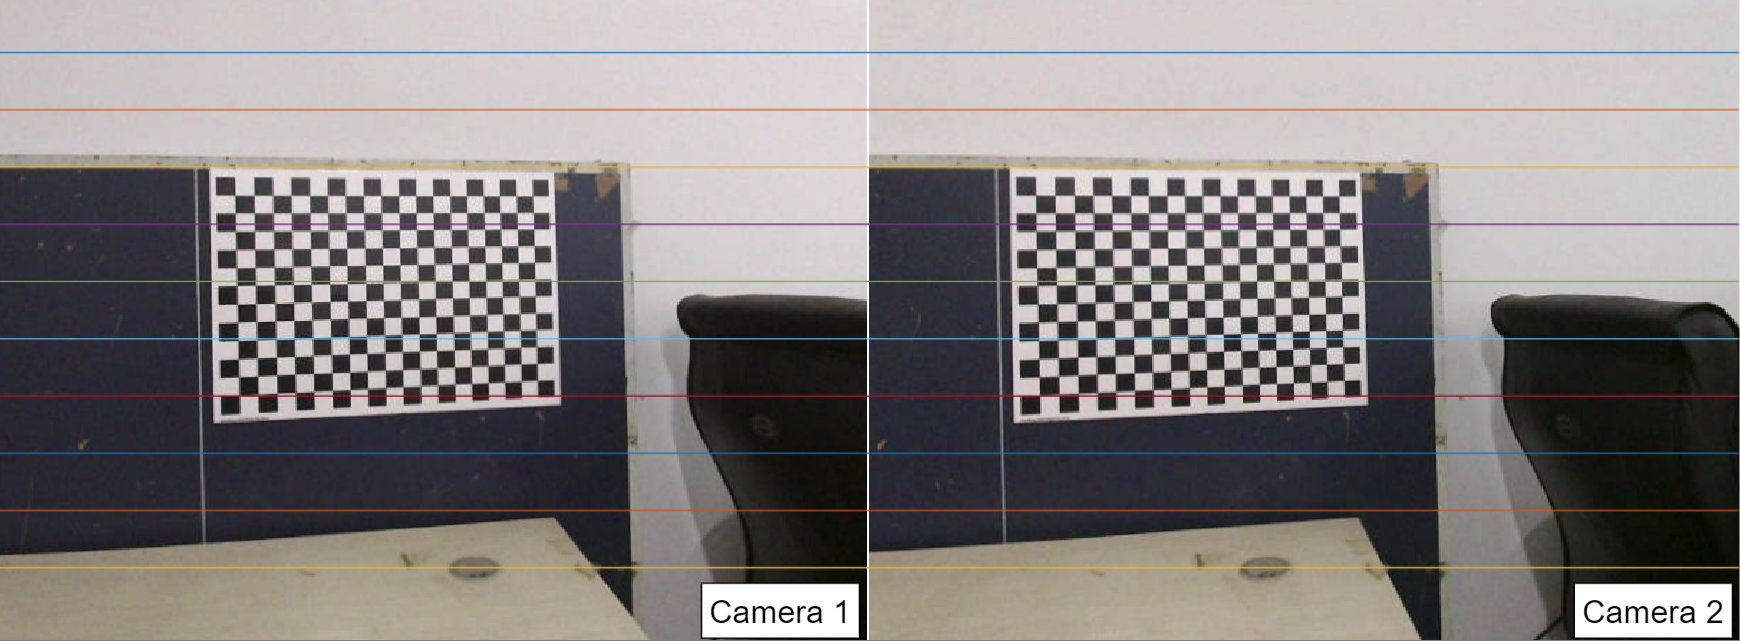
\includegraphics[width=0.95\textwidth]{figures/chapter03/图像校正处理结果.png}
  \caption{图像校正处理结果}
  \label{图像校正处理结果}
\end{figure}

\subsection{轻量化立体匹配模型}

现有轻量化立体匹配研究主要围绕降低代价建模与聚合开销展开：StereoNet\cite{khamisStereonetGuidedHierarchical2018a}通过低分辨率匹配表示并结合逐级细化实现粗到细估计，AANet\cite{xuAANetAdaptiveAggregation2020}采用自适应聚合在多尺度上动态调制代价融合，MobileNetStereo-2D\cite{shamsafarMobilestereonetLightweightDeep2022a}以轻量化骨干配合二维聚合策略压缩计算量，HITNet\cite{tankovichHitnetHierarchicalIterative2021a}通过假设驱动的迭代推理逐步优化视差以减少对显式重型代价正则化的依赖，Fast-ACVNet\cite{xuAccurateEfficientStereo2023}与IINet\cite{liIinetImplicitIntrainter2024}则分别从高效代价体构建/聚合与左右特征交互优化角度提升信息利用效率。尽管上述方法在实时性方面取得进展，但在轻量化约束下，代价体构建阶段对多尺度几何信息的利用往往仍较为有限，粗尺度几何先验对细尺度匹配的引导作用仍有进一步挖掘空间。

针对上述问题，本文设计了轻量化立体匹配模型HAGVNet。该模型以分层注意力引导代价体HAGV（Hierarchical Attention-Guided Cost Volume）为核心，通过粗尺度几何先验调制细尺度代价建模过程，并结合轻量化的ConvNeXtV2\cite{wooConvnextV2Codesigning2023a}风格二维代价聚合模块，在保证计算复杂度可控的前提下提升匹配精度与场景鲁棒性，其整体结构如图\ref{HAGVNet结构图}所示。

\begin{figure}[h]
  \centering
  \includesvg[width=1\textwidth]{figures/chapter03/HAGVNet结构图}
  \caption{HAGVNet结构图}
  \label{HAGVNet结构图}
\end{figure}

（1）分层注意力引导代价体构建

与直接在单尺度上构建代价体的方法不同，本文在代价建模阶段显式引入粗尺度几何先验，对细尺度代价体进行调制。传统轻量化立体匹配模型通常仅依赖单尺度特征构建相关性代价体，缺乏来自粗尺度几何结构的约束，在弱纹理、重复纹理及遮挡区域易导致代价分布不稳定。为提升细尺度匹配的稳定性与几何一致性，本文提出分层注意力引导的代价体构建方法（Hierarchical Attention-Guided Cost Volume, HAGV）。该方法首先在粗尺度上获取稳定的几何先验，并将其作为一种弱几何约束前置到代价体构建阶段，用于调制细尺度代价建模过程。由此，使细尺度代价体在生成阶段即具备一定的几何一致性，而非仅依赖后续聚合阶段进行补偿，从而为后续代价聚合与视差回归提供更稳定、物理约束更强的输入。

在该流程中，模型由骨干网络提取左右图像的多尺度特征，并分别利用原图$1/8$分辨率与$1/4$分辨率特征构建粗尺度代价体与细尺度代价体。粗尺度代价体经轻量聚合与视差回归后得到粗尺度视差先验$d_{\text{coarse}}$，随后将$d_{\text{coarse}}$上采样至细尺度，并据此生成平滑的高斯注意力先验。高斯注意力形式见式~\eqref{eq:ch3-attention}：
\begin{equation}\label{eq:ch3-attention}
A=\exp\left(-\frac{(d_{\text{coarse}}-\mu)^2}{2\sigma^2}\right)
\end{equation}
\begin{tabularx}{\textwidth}{@{}l@{\quad}r@{———}X@{}}
式中& $A$ & 分层注意力先验权重；\\
& $d_{\text{coarse}}$ & 粗尺度视差先验；\\
& $\mu$ & 以粗尺度先验为中心的局部均值；\\
& $\sigma$ & 尺度相关的平滑系数。\\
\end{tabularx}\vspace{3.15bp}

随后利用注意力先验对细尺度代价体$C_{\text{fine}}$进行调制，并由轻量级卷积分支提取残差信息$\Delta C$，加性残差融合形式如式~\eqref{eq:ch3-fusion}所示：
\begin{equation}\label{eq:ch3-fusion}
C'_{\text{fine}}=C_{\text{fine}}+A\odot\Delta C
\end{equation}
\begin{tabularx}{\textwidth}{@{}l@{\quad}r@{———}X@{}}
式中& $C'_{\text{fine}}$ & 融合后的细尺度代价体；\\
& $C_{\text{fine}}$ & 细尺度代价体；\\
& $\Delta C$ & 由轻量级卷积分支提取的残差信息；\\
& $\odot$ & 逐通道逐元素乘法。\\
\end{tabularx}\vspace{3.15bp}

该机制赋予几何可靠区域更高权重，抑制不确定区域，使代价体在构建阶段即具备更强的几何一致性，从而提升聚合阶段的匹配稳定性与边界一致性。

（2）用于2D代价聚合的ConvNeXtV2聚合块

先前的二维代价聚合研究多以轻量卷积结构为核心，通过深度可分离卷积与倒置残差块（如MobileNet系列\cite{sandlerMobilenetv2InvertedResiduals2018}）在聚合阶段压缩计算开销。相关思路已在MobileNetStereo-2D\cite{shamsafarMobilestereonetLightweightDeep2022a}以及以MobileNetV2\cite{sandlerMobilenetv2InvertedResiduals2018}为骨干的LightStereo\cite{guoLightstereoChannelBoost2025}中得到验证，表明该类方法在嵌入式算力受限场景下表现出较好的速度-精度折中特性。然而，此类以局部卷积运算为主的轻量结构在建模长程空间依赖及复杂几何关系方面仍存在一定局限，易导致代价聚合阶段的特征表征能力受限。基于上述考虑，本文在二维代价聚合网络中引入ConvNeXtV2\cite{wooConvnextV2Codesigning2023a}风格的轻量残差块，在保持整体计算复杂度可控的前提下，通过大核卷积、规范化与非线性激活的协同设计增强空间与通道维度的表达能力，从而提升聚合特征对复杂匹配模式的建模能力。其整体结构示意如图\ref{不同代价卷积块对比}(d)所示。

\begin{figure}[h]
  \centering
  \includesvg[width=0.90\textwidth]{figures/chapter03/不同代价卷积块对比}
  \caption{不同代价卷积块对比}
  \label{不同代价卷积块对比}
\end{figure}

设输入代价体为$X$。该模块首先通过深度卷积$DWConv$扩大感受野，以增强对局部上下文的建模能力，如式~\eqref{eq:ch3-conv1}所示：
\begin{equation}\label{eq:ch3-conv1}
X_1=DWConv_{7\times 7}(X)
\end{equation}
\begin{tabularx}{\textwidth}{@{}l@{\quad}r@{———}X@{}}
式中& $X$ & 输入代价体；\\
& $X_1$ & 深度卷积后的特征；\\
& DWConv & 深度卷积操作。\\
\end{tabularx}\vspace{3.15bp}

随后对特征施加二维层归一化$LN$以稳定训练过程，如式~\eqref{eq:ch3-ln}所示：
\begin{equation}\label{eq:ch3-ln}
X_2=LN(X_1)
\end{equation}
\begin{tabularx}{\textwidth}{@{}l@{\quad}r@{———}X@{}}
式中& $X_2$ & 经层归一化后的特征；\\
& $LN$ & 二维层归一化操作。\\
\end{tabularx}\vspace{3.15bp}

在此基础上，采用逐点卷积$W_1$进行通道扩张，并引入 GELU 非线性激活，如式~\eqref{eq:ch3-gelu}所示：
\begin{equation}\label{eq:ch3-gelu}
X_3=GELU(W_1*X_2)
\end{equation}
\begin{tabularx}{\textwidth}{@{}l@{\quad}r@{———}X@{}}
式中& $X_3$ & 经通道扩张和非线性激活后的特征；\\
& $W_1$ & 逐点卷积权重，用于通道扩张；\\
& GELU & 高斯误差线性单元激活函数。\\
\end{tabularx}\vspace{3.15bp}

为进一步调节通道维度上的全局响应，引入 Global Response Normalization（GRN）模块，如式~\eqref{eq:ch3-grn}所示：
\begin{equation}\label{eq:ch3-grn}
X_4=GRN(X_3)
\end{equation}
\begin{tabularx}{\textwidth}{@{}l@{\quad}r@{———}X@{}}
式中& $X_4$ & 经全局响应归一化后的特征；\\
& GRN & 全局响应归一化操作。\\
\end{tabularx}\vspace{3.15bp}

随后通过另一个卷积将通道数映射回原始维度，如式~\eqref{eq:ch3-conv2}所示：
\begin{equation}\label{eq:ch3-conv2}
X_5=W_2*X_4
\end{equation}
\begin{tabularx}{\textwidth}{@{}l@{\quad}r@{———}X@{}}
式中& $X_5$ & 投影卷积后的输出特征；\\
& $W_2$ & 投影卷积权重，用于将通道数映射回原始维度。\\
\end{tabularx}\vspace{3.15bp}

当输入与输出特征维度一致时，引入残差连接以缓解梯度消失并增强特征复用能力，如式~\eqref{eq:ch3-res}所示：
\begin{equation}\label{eq:ch3-res}
Y=X+X_5
\end{equation}
\begin{tabularx}{\textwidth}{@{}l@{\quad}r@{———}X@{}}
式中& $Y$ & 残差融合后的输出特征。\\
\end{tabularx}\vspace{3.15bp}

该ConvNeXtV2风格残差块通过大核深度卷积、通道扩张、归一化与残差融合的组合设计，在维持轻量化特性的同时显著增强了模型对平面区域与边界纹理的建模能力，适用于对精度与算力均有约束的嵌入式立体匹配场景。对比实验结果表明，该结构在综合性能上优于ShuffleNet-V2、GhostNet\cite{hanGhostnetMoreFeatures2020a}及MobileNet-V2\cite{sandlerMobilenetv2InvertedResiduals2018}等常见轻量残差块。

（3）网络整体结构

综合上述设计，本文提出的HAGVNet主要由特征提取、代价体构建、代价聚合、视差回归和损失函数五个部分组成。

1）多尺度特征提取

设输入左右图像分别为$I_l$与$I_r$。本文采用在ImageNet\cite{dengImagenetLargescaleHierarchical2009a}上预训练的MobileNetV2\cite{sandlerMobilenetv2InvertedResiduals2018}作为骨干网络，对输入图像进行逐级下采样以提取多尺度结构与纹理特征。在骨干网络输出的基础上，引入双向特征金字塔（BiFPN\cite{tanEfficientdetScalableEfficient2020b}），用于在高、低分辨率特征之间进行有效的信息融合，从而增强多尺度几何结构的一致性。最终在$1/4$与$1/8$分辨率下分别获得左右图像的特征图，并分别用于细尺度与粗尺度代价体的构建。

2）代价体构建

设用于构建代价体的左右特征分别为$F_l$和$F_r$，对应的视差搜索范围为$d\in[0,D_{\max}-1]$。在该范围内，对于每个视差$d$，将右特征在水平方向平移$d$个像素，并与左特征逐通道计算归一化相似度。代价体定义如式~\eqref{eq:ch3-cost}所示：
\begin{equation}\label{eq:ch3-cost}
C(x,y,d)=\frac{1}{N_s}\left\langle F_l(x,y),F_r(x-d,y)\right\rangle
\end{equation}
\begin{tabularx}{\textwidth}{@{}l@{\quad}r@{———}X@{}}
式中& $C(x,y,d)$ & 像素$(x,y)$在视差$d$处的匹配代价值；\\
& $F_l,\,F_r$ & 左右图像对应尺度下的特征图；\\
& $\left\langle \cdot,\cdot \right\rangle$ & 两个特征向量的内积运算；\\
& $N_s$ & 特征通道数。\\
\end{tabularx}\vspace{3.15bp}

利用1/4分辨率特征构建细尺度代价体，利用1/8分辨率特征构建粗尺度代价体。粗尺度代价体用于提供更大感受野下的全局匹配先验，细尺度代价体则保留更多边缘和局部结构信息，二者互补以提升复杂区域的匹配稳定性。

最后应用3.1节所述的分层注意力引导代价机制构建融合后的代价体。

3）代价聚合

代价聚合阶段分别对粗尺度代价体与细尺度代价体进行层次化聚合，二者采用相同的 ConvNeXtV2 风格残差块。两条聚合分支仅在输入分辨率与通道数上存在差异。每条分支均以输入代价体为起点，逐级进行 1/2 与 1/4 下采样，并结合 U-Net 式对称上采样和跨尺度跳连融合多层级信息，从而增强代价体的空间一致性与几何关联性，其整体结构如图\ref{代价聚合结构图}所示。

\begin{figure}[h]
  \centering
  \includesvg[width=1\textwidth]{figures/chapter03/代价聚合结构图}
  \caption{代价聚合结构图}
  \label{代价聚合结构图}
\end{figure}

4）视差回归

在完成代价聚合后，对代价体采用soft-argmax操作预测最终视差图。具体而言，首先对每个像素位置处所有视差对应的代价值施加softmax归一化，得到视差概率分布$p$，如式~\eqref{eq:ch3-prob}所示：
\begin{equation}\label{eq:ch3-prob}
p(d\mid x,y)=\frac{\exp[-C(x,y,d)]}{\sum_{k=0}^{D_{\max}-1}\exp[-C(x,y,k)]}
\end{equation}
\begin{tabularx}{\textwidth}{@{}l@{\quad}r@{———}X@{}}
式中& $p(d\mid x,y)$ & 像素$(x,y)$处视差为$d$的概率；\\
& $D_{\max}$ & 最大搜索视差；\\
& $k$ & 视差求和索引。\\
\end{tabularx}\vspace{3.15bp}

然后对离散视差值按该概率分布加权求和，得到像素$(x,y)$处的视差回归值$d(x,y)$，如式~\eqref{eq:ch3-disp-reg}所示：
\begin{equation}\label{eq:ch3-disp-reg}
d(x,y)=\sum_{k=0}^{D_{\max}-1} k\cdot p(k\mid x,y)
\end{equation}
\begin{tabularx}{\textwidth}{@{}l@{\quad}r@{———}X@{}}
式中& $d(x,y)$ & 像素$(x,y)$处的视差回归值。\\
\end{tabularx}\vspace{3.15bp}

5）损失函数

首先定义单尺度视差预测的基本损失形式。设预测视差为$d$，真实视差为$d^*$，在共有$N$个有效像素的位置上，采用Smooth L1损失度量二者之间的差异，如式~\eqref{eq:ch3-loss-single}所示：
\begin{equation}\label{eq:ch3-loss-single}
L(d,d^*)=\frac{1}{N}\sum_{i=1}^{N}\mathrm{SmoothL1}(d_i-d_i^*)
\end{equation}
\begin{tabularx}{\textwidth}{@{}l@{\quad}r@{———}X@{}}
式中& $L(d,d^*)$ & 单尺度视差监督损失；\\
& $d$ & 预测视差；\\
& $d^*$ & 真实视差；\\
& $N$ & 有效像素总数；\\
& $d_i$ & 第$i$个像素的预测视差；\\
& $d_i^*$ & 第$i$个像素的真实视差。\\
\end{tabularx}\vspace{3.15bp}

在此基础上，模型采用粗尺度与最终尺度的联合监督策略，以进一步提升几何一致性与训练稳定性。设最终尺度视差预测为$d$，粗尺度视差预测为$d_{\text{coarse}}$，则联合损失写为式~\eqref{eq:ch3-loss-total}：
\begin{equation}\label{eq:ch3-loss-total}
L_{\text{total}}=L(d,d^*)+\lambda L(d_{\text{coarse}},d^*)
\end{equation}
\begin{tabularx}{\textwidth}{@{}l@{\quad}r@{———}X@{}}
式中& $L_{\text{total}}$ & 联合监督总损失；\\
& $L(\cdot)$ & 单尺度视差监督损失；\\
& $\lambda$ & 粗尺度监督损失的权重系数。\\
\end{tabularx}\vspace{3.15bp}

该联合监督项在训练阶段用于引入额外的几何先验约束。

综上，本文提出的HAGVNet围绕粗尺度几何先验引导细尺度匹配这一核心思路，对代价体构建、聚合与监督方式进行了统一设计。其中，HAGV模块用于增强弱纹理、重复纹理及遮挡区域的匹配稳定性，ConvNeXtV2风格聚合块用于在有限计算开销下提升特征表达能力，联合监督策略则进一步保证训练过程的稳定性。上述设计共同构成了本文双目感知模块的核心基础，并为后续训练配置、消融实验、对比分析以及整车测距应用提供了方法支撑。

\subsection{立体匹配模型的训练及评价指标}
\label{sec:ch3-stereo-training-metrics}

为验证上述轻量化立体匹配模型的有效性与泛化能力，本文采用“合成数据预训练+真实数据微调”的两阶段训练策略，并结合主流评价指标对模型性能进行定量分析。相关训练配置与评价标准不仅用于考察模型的匹配性能，也作为后文消融实验、对比实验及嵌入式部署分析的统一实验依据。模型训练与测试均在统一软硬件环境下进行，实验平台为Windows 11操作系统、NVIDIA GeForce RTX 4090显卡和Intel Core i5-9600KF处理器，深度学习框架为PyTorch 1.9，编程语言为Python 3.8。

（1）预训练阶段

模型首先在 SceneFlow 数据集\cite{mayerLargeDatasetTrain2016}上进行预训练。SceneFlow 是面向视差、光流与场景流估计的大规模合成双目数据集，具有稠密、精确的像素级视差真值，可为模型提供充分的几何监督，常用于立体匹配网络的预训练。预训练阶段采用端点误差（End-Point Error, EPE）为主要评价指标，其定义如式~\eqref{eq:ch3-epe}所示：
\begin{equation}\label{eq:ch3-epe}
\mathrm{EPE}=\frac{1}{N}\sum_{i=1}^{N}\left|d_i^{pred}-d_i^{gt}\right|
\end{equation}
\begin{tabularx}{\textwidth}{@{}l@{\quad}r@{———}X@{}}
式中& $\mathrm{EPE}$ & 端点误差评价指标；\\
& $N$ & 有效像素总数；\\
& $d_i^{pred}$ & 第$i$个像素的预测视差；\\
& $d_i^{gt}$ & 第$i$个像素对应的真实视差。\\
\end{tabularx}\vspace{3.15bp}

EPE实质为像素级视差绝对误差的平均值，能够直接反映整体匹配精度。预训练阶段批量大小设为12，优化器采用AdamW，学习率调度策略为OneCycleLR，共训练90个轮次，数据增强方式以随机裁剪为主。

（2）微调与测试阶段

完成预训练后，模型在 KITTI 2012\cite{geigerAreWeReady2012a} 与 KITTI 2015\cite{menzeObjectSceneFlow2015a} 混合数据集上进行微调与测试。KITTI 数据集来源于车载平台采集的真实道路场景，包含实际光照、遮挡、反射以及动态交通目标等因素，更贴近自动驾驶与移动机器人应用需求，因此适合检验模型从合成数据迁移到真实环境后的泛化能力。在 KITTI 2012 中，仍采用EPE作为评价指标，在 KITTI 2015 中，采用D1-all指标，其定义如式~\eqref{eq:ch3-d1all}所示：
\begin{equation}\label{eq:ch3-d1all}
\mathrm{D1}\text{-all}=\frac{\left|\left\{i:\left|d_i^{pred}-d_i^{gt}\right|>3\ \text{or}\ \frac{\left|d_i^{pred}-d_i^{gt}\right|}{d_i^{gt}}>0.05\right\}\right|}{N}\times 100\%
\end{equation}
\begin{tabularx}{\textwidth}{@{}l@{\quad}r@{———}X@{}}
式中& $\left|\left\{\cdot\right\}\right|$ & 满足误差条件的像素集合元素个数；\\
& $N$ & 有效像素总数；\\
& $3$ & 绝对误差阈值（像素）；\\
& $0.05$ & 相对误差阈值（5\%）。\\
\end{tabularx}\vspace{3.15bp}

D1-all反映大误差像素比例，能够更有效评估模型在遮挡、弱纹理及动态场景下的鲁棒性。

微调阶段训练500个轮次，批量大小设为2，继续采用OneCycleLR调度策略。同时引入颜色抖动、随机擦除、随机缩放与随机裁剪等数据增强方法，以提升模型对复杂真实环境的适应能力。

为统一衡量模型的计算复杂度，本文采用单次前向传播中的浮点运算次数（FLOPs）作为复杂度指标。对于卷积层，其计算方式定义如式~\eqref{eq:ch3-flops}所示：
\begin{equation}\label{eq:ch3-flops}
\mathrm{FLOPs}=2\times H\times W\times C_{\mathrm{in}}\times C_{\mathrm{out}}\times \frac{k_h\times k_w}{\mathrm{groups}}
\end{equation}
\begin{tabularx}{\textwidth}{@{}l@{\quad}r@{———}X@{}}
式中& $\mathrm{FLOPs}$ & 单次前向传播中的浮点运算次数；\\
& $H, W$ & 输出特征图的空间高度与宽度；\\
& $C_{\mathrm{in}}, C_{\mathrm{out}}$ & 输入与输出通道数；\\
& $k_h, k_w$ & 卷积核的高度与宽度；\\
& $\mathrm{groups}$ & 分组卷积的组数。\\
\end{tabularx}\vspace{3.15bp}

\subsection{立体匹配模型实验结果与分析}

为评估所提出立体匹配模型的精度--复杂度权衡性能，本节从轻量化卷积块选择、HAGV模块有效性及与主流方法对比三个方面展开实验分析。

（1）卷积块消融实验

在保持网络结构与训练策略一致的条件下，对不同风格的卷积块在SceneFlow数据集\cite{mayerLargeDatasetTrain2016}上进行了对比实验，其结果如表\ref{不同卷积块在SceneFlow数据集上的消融实验}所示。ShuffleNetV2与GhostNet\cite{hanGhostnetMoreFeatures2020a}在FLOPs与参数规模方面最为轻量（FLOPs约17.9G，参数量低于3M），但匹配精度相对较低，其EPE分别为0.9223与0.8271，表明其在弱纹理与复杂几何区域的特征表达能力受限。相比之下，ConvNeXtV2\cite{wooConvnextV2Codesigning2023a}在FLOPs为19.58G、参数量为3.40M的条件下取得最低的EPE（0.7644），且相较MobileNetV2\cite{sandlerMobilenetv2InvertedResiduals2018}，EPE下降约3.7\%；相较GhostNet与ShuffleNetV2，误差分别降低约7.6\%与17.1\%。综合考虑精度、计算量与模型规模，ConvNeXtV2在当前实验配置下实现了更优的精度–复杂度折中，因此被选作后续实验的基础代价聚合单元。

\begin{table}[htbp]
  \centering
  \caption[不同卷积块在SceneFlow数据集上的消融实验]{不同卷积块在SceneFlow数据集上的消融实验}
  \label{不同卷积块在SceneFlow数据集上的消融实验}
  \vspace{0.5em}\wuhao
  \begin{thesistabular}{cccc}
    \toprule
    卷积块类型 & FLOPs(G) & Params(M) & EPE \\
    \midrule
    GhostNet & 17.94 & 2.82 & 0.8271 \\
    ShuffleNetV2 & 17.93 & 2.65 & 0.9223 \\
    MobileNetV2 & 20.32 & 3.44 & 0.7935 \\
    ConvNeXtV2 & 19.58 & 3.40 & 0.7644 \\
    \bottomrule
  \end{thesistabular}
\end{table}
\FloatBarrier

（2）HAGV模块消融实验

为验证分层注意力引导代价体（HAGV）模块的有效性，本文在以ConvNeXtV2为基本卷积单元的基础上，对是否引入HAGV及不同粗尺度设置进行了消融实验，结果如表\ref{HAGV模块在SceneFlow数据集上的消融实验}所示。基线模型仅利用1/4分辨率特征进行代价建模，其EPE为0.7644。引入HAGV后，模型精度进一步提升：当粗尺度分支设为1/16时，EPE降至0.7612；当粗尺度分支设为1/8时，EPE进一步降至0.7415，而FLOPs仅由19.58G增至20.08G。结果表明，HAGV通过引入粗尺度几何先验增强了代价体的几何一致性与匹配稳定性，其中1/8分辨率粗尺度分支取得了更优的精度--复杂度折中。

\begin{table}[htbp]
  \centering
  \caption[HAGV模块在SceneFlow数据集上的消融实验]{HAGV模块在SceneFlow数据集上的消融实验}
  \label{HAGV模块在SceneFlow数据集上的消融实验}
  \vspace{0.5em}\wuhao
  \begin{thesistabular}{cccccc}
    \toprule
    配置 & 粗尺度 & 细尺度 & FLOPs(G) & Params(M) & epe \\
    \midrule
    Baseline & - & 1/4 & 19.58 & 3.40 & 0.7644 \\
    +HAGV & 1/16 & 1/4 & 19.61 & 3.50 & 0.7612 \\
    +HAGV & 1/8 & 1/4 & 20.08 & 3.78 & 0.7415 \\
    \bottomrule
  \end{thesistabular}
\end{table}

（3）与主流方法的对比实验

为进一步验证模型的整体性能，本文在SceneFlow\cite{mayerLargeDatasetTrain2016}与KITTI数据集\cite{geigerAreWeReady2012a,menzeObjectSceneFlow2015a}上将所提出的HAGVNet与多种主流实时或轻量化立体匹配方法进行对比，结果分别如表\ref{在SceneFlow数据集上对比其他主流实时立体匹配网络}和表\ref{在KITTI数据集上对比其他主流轻量立体匹配网络}所示。其中，KITTI数据集结果由官方评测服务器获得。为消除硬件差异，统一采用FLOPs作为计算复杂度指标，在1242×375分辨率下统计。对比方法包括StereoNet\cite{khamisStereonetGuidedHierarchical2018a}、DeepPrunerFast\cite{duggalDeepprunerLearningEfficient2019a}、AANet\cite{xuAANetAdaptiveAggregation2020}、HITNet\cite{tankovichHitnetHierarchicalIterative2021a}、CoEx\cite{bangunharcanaCorrelateandexciteRealtimeStereo2021a}、MobileStereoNet-2D\cite{shamsafarMobilestereonetLightweightDeep2022a}、Fast-ACVNet/Fast-ACVNet+\cite{xuAccurateEfficientStereo2023}与IINet\cite{liIinetImplicitIntrainter2024}等代表性方法。

\begin{figure}[h]
  \centering
  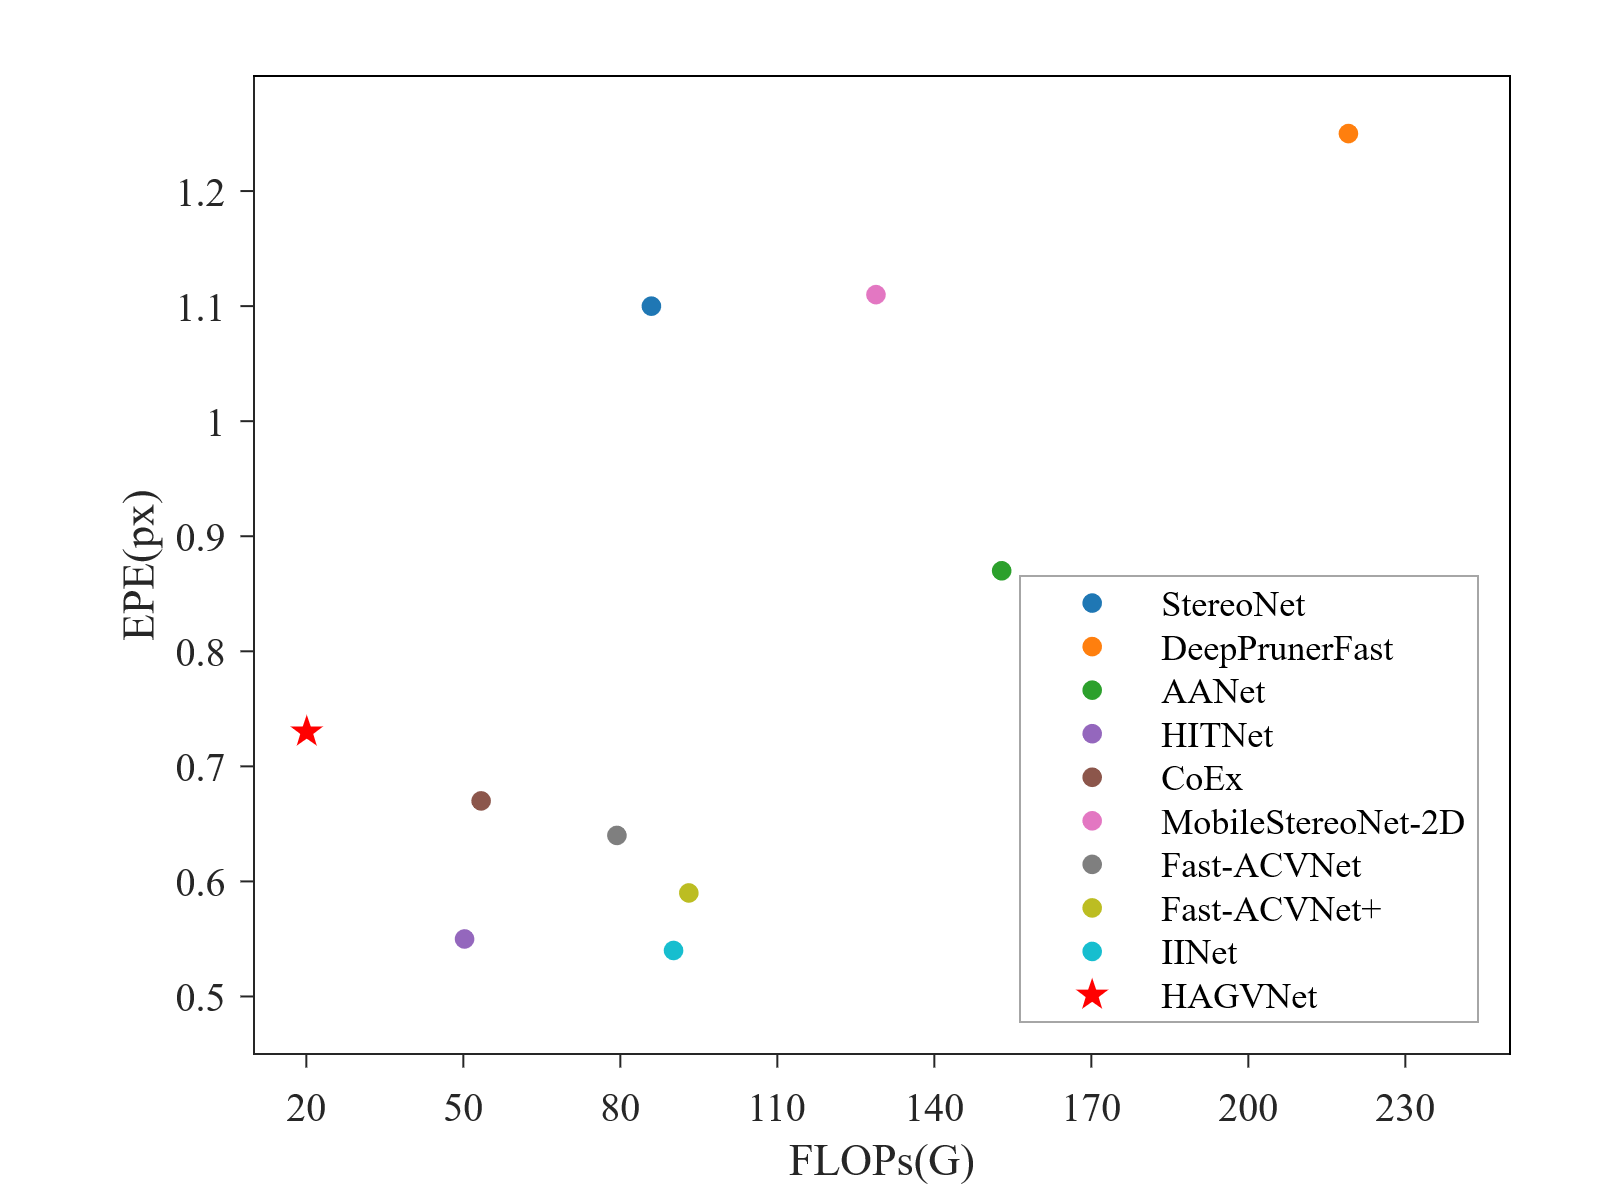
\includegraphics[width=0.95\textwidth]{figures/chapter03/SceneFlow性能与FLOPs对比.png}
  \caption{SceneFlow数据集上的性能与FLOPs对比}
  \label{SceneFlow数据集上的性能与FLOPs对比}
\end{figure}

\begin{figure}[h]
  \centering
  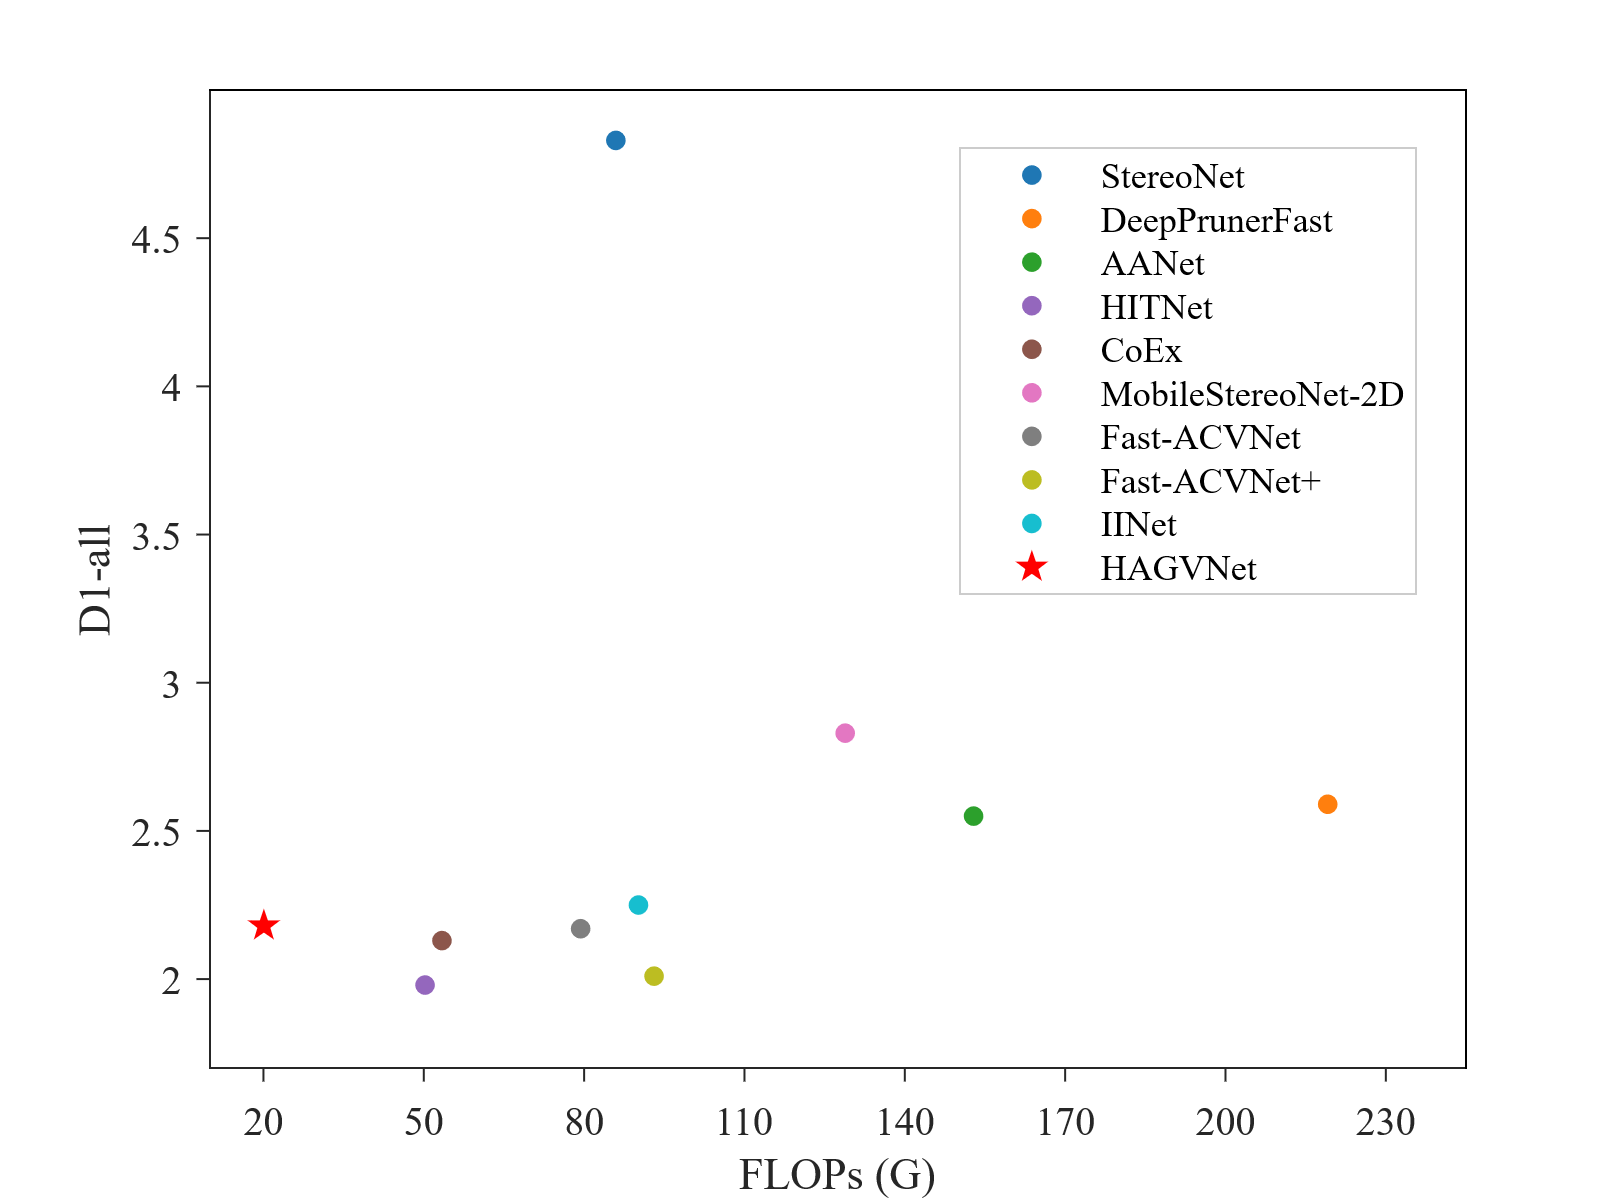
\includegraphics[width=0.95\textwidth]{figures/chapter03/KITTI2015性能与FLOPs对比.png}
  \caption{KITTI 2015数据集上的性能与FLOPs对比}
  \label{KITTI2015数据集上的性能与FLOPs对比}
\end{figure}
\FloatBarrier

在SceneFlow数据集上，HAGVNet在仅$20.08\,\mathrm{GFLOPs}$的条件下取得$0.73\,\mathrm{px}$的EPE，在计算量显著低于多数方法的情况下保持了具有竞争力的精度表现，其精度与复杂度关系如图\ref{SceneFlow数据集上的性能与FLOPs对比}所示；在KITTI 2012与KITTI 2015数据集上，HAGVNet的整体性能优于StereoNet\cite{khamisStereonetGuidedHierarchical2018a}、DeepPrunerFast\cite{duggalDeepprunerLearningEfficient2019a}、MobileStereoNet-2D\cite{shamsafarMobilestereonetLightweightDeep2022a}与AANet\cite{xuAANetAdaptiveAggregation2020}等方法。与HITNet\cite{tankovichHitnetHierarchicalIterative2021a}及Fast-ACVNet系列\cite{xuAccurateEfficientStereo2023}相比，HAGVNet在D1-all指标上仅高出约0.2\%--0.3\%，但其计算复杂度仅为$20.08\,\mathrm{GFLOPs}$，分别约为HITNet（$50.23\,\mathrm{GFLOPs}$）的40\%和Fast-ACVNet（$79.34\,\mathrm{GFLOPs}$）的25\%，在保持接近精度的同时显著降低了计算开销，其在KITTI 2015数据集上的性能与FLOPs关系如图\ref{KITTI2015数据集上的性能与FLOPs对比}所示。图\ref{HAGVNet与多种主流方法在KITTI数据集上的部分表现}给出了部分定性结果对比，可见在弱纹理区域与大面积平坦区域，HAGVNet能较好保持结构连续性并抑制局部匹配噪声。

\begin{figure}[h]
  \centering
  \begin{minipage}[b]{0.245\textwidth}
    \centering
    
\includegraphics[width=\linewidth,height=0.16\textheight,keepaspectratio]{figures/chapter03/Qualitative_comparison/Qualitative_comparison1_1}
    \vspace{2mm}
    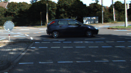
\includegraphics[width=\linewidth,height=0.16\textheight,keepaspectratio]{figures/chapter03/Qualitative_comparison/Qualitative_comparison1_2}
    \vspace{2mm}
    \small (a) 左图
  \end{minipage}\hfill
  \begin{minipage}[b]{0.245\textwidth}
    \centering
    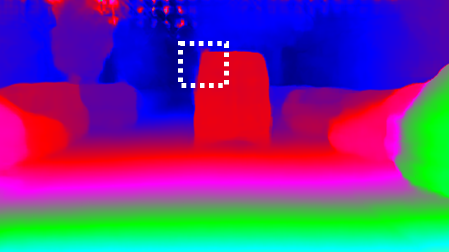
\includegraphics[width=\linewidth,height=0.16\textheight,keepaspectratio]{figures/chapter03/Qualitative_comparison/Qualitative_comparison2_1}
    \vspace{2mm}
    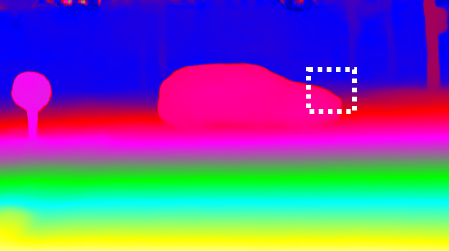
\includegraphics[width=\linewidth,height=0.16\textheight,keepaspectratio]{figures/chapter03/Qualitative_comparison/Qualitative_comparison2_2}
    \vspace{2mm}
    \small (b) HAGVNet（本文）
  \end{minipage}\hfill
  \begin{minipage}[b]{0.245\textwidth}
    \centering
    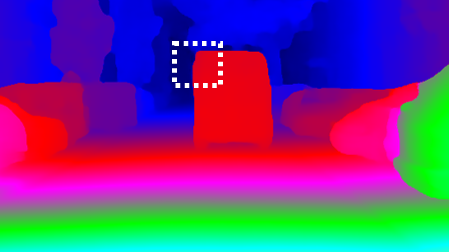
\includegraphics[width=\linewidth,height=0.16\textheight,keepaspectratio]{figures/chapter03/Qualitative_comparison/Qualitative_comparison3_1}
    \vspace{2mm}
    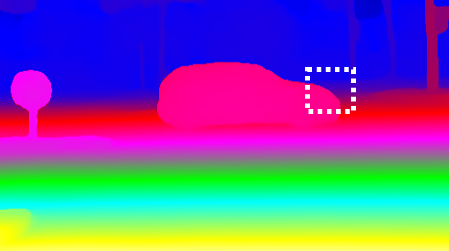
\includegraphics[width=\linewidth,height=0.16\textheight,keepaspectratio]{figures/chapter03/Qualitative_comparison/Qualitative_comparison3_2}
    \vspace{2mm}
    \small (c) MobileStereoNet-2D
  \end{minipage}\hfill
  \begin{minipage}[b]{0.245\textwidth}
    \centering
    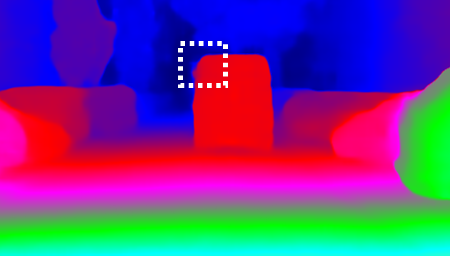
\includegraphics[width=\linewidth,height=0.16\textheight,keepaspectratio]{figures/chapter03/Qualitative_comparison/Qualitative_comparison4_1}
    \vspace{2mm}
    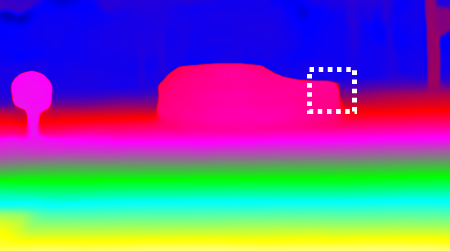
\includegraphics[width=\linewidth,height=0.16\textheight,keepaspectratio]{figures/chapter03/Qualitative_comparison/Qualitative_comparison4_2}
    \vspace{2mm}
    \small (d) HITNet
  \end{minipage}
  \caption{HAGVNet与多种主流方法在KITTI数据集上的部分表现}
  \label{HAGVNet与多种主流方法在KITTI数据集上的部分表现}
\end{figure}

\begin{table}[htbp]
  \centering
  \caption[在SceneFlow数据集上对比其他主流实时立体匹配网络]{在SceneFlow数据集上对比其他主流实时立体匹配网络}
  \label{在SceneFlow数据集上对比其他主流实时立体匹配网络}
  \vspace{0.5em}\wuhao
  \begin{thesistabular}{cccc}
    \toprule
    方法 & FLOPs (G) & Params (M) & EPE (px) \\
    \midrule
    StereoNet\cite{khamisStereonetGuidedHierarchical2018a} & 85.93 & 0.40 & 1.10 \\
    DeepPrunerFast\cite{duggalDeepprunerLearningEfficient2019a} & 219.12 & 7.47 & 1.25 \\
    AANet\cite{xuAANetAdaptiveAggregation2020} & 152.86 & 2.97 & 0.87 \\
    HITNet\cite{tankovichHitnetHierarchicalIterative2021a} & 50.23 & 0.42 & 0.55 \\
    CoEx\cite{bangunharcanaCorrelateandexciteRealtimeStereo2021a} & 53.39 & 2.72 & 0.67 \\
    MobileStereoNet-2D\cite{shamsafarMobilestereonetLightweightDeep2022a} & 128.84 & 2.23 & 1.11 \\
    Fast-ACVNet\cite{xuAccurateEfficientStereo2023} & 79.34 & 3.08 & 0.64 \\
    Fast-ACVNet+\cite{xuAccurateEfficientStereo2023} & 93.08 & 3.20 & 0.59 \\
    IINet\cite{liIinetImplicitIntrainter2024} & 90.16 & 19.54 & 0.54 \\
    HAGVNet（ours） & 20.08 & 3.78 & 0.73 \\
    \bottomrule
  \end{thesistabular}
\end{table}

\begin{table}[htbp]
  \centering
  \caption[在KITTI数据集上对比其他主流轻量立体匹配网络]{在KITTI数据集上对比其他主流轻量立体匹配网络}
  \label{在KITTI数据集上对比其他主流轻量立体匹配网络}
  \vspace{0.5em}\wuhao
  \begingroup
  \setlength{\tabcolsep}{3pt}
  \begin{thesistabular}{ccccccccc}
    \toprule
    \multirow{2}{*}{方法} & \multicolumn{4}{c}{KITTI 2012} & \multicolumn{3}{c}{KITTI 2015} & \multirow{2}{*}{FLOPs(G)} \\
    \cmidrule(lr){2-5}\cmidrule(lr){6-8}
     & 3-noc & 3-all & 4-noc & 4-all & D1-bg & D1-fg & D1-all &  \\
    \midrule
    StereoNet\cite{khamisStereonetGuidedHierarchical2018a} & - & - & - & - & 4.30 & 7.45 & 4.83 & 85.93 \\
    DeepPrunerFast\cite{duggalDeepprunerLearningEfficient2019a} & - & - & - & - & 2.32 & 3.91 & 2.59 & 219.12 \\
    AANet\cite{xuAANetAdaptiveAggregation2020} & 1.91 & 2.42 & 1.46 & 1.87 & 1.99 & 5.39 & 2.55 & 152.86 \\
    HITNet\cite{tankovichHitnetHierarchicalIterative2021a} & 1.41 & 1.89 & 1.14 & 1.53 & 1.74 & 3.20 & 1.98 & 50.23 \\
    CoEx\cite{bangunharcanaCorrelateandexciteRealtimeStereo2021a} & 1.55 & 1.93 & 1.15 & 1.42 & 1.79 & 3.82 & 2.13 & 53.39 \\
    MobileStereoNet-2D\cite{shamsafarMobilestereonetLightweightDeep2022a} & - & - & - & - & 2.49 & 4.53 & 2.83 & 128.84 \\
    Fast-ACVNet\cite{xuAccurateEfficientStereo2023} & 1.68 & 2.13 & 1.23 & 1.56 & 1.82 & 3.93 & 2.17 & 79.34 \\
    Fast-ACVNet+\cite{xuAccurateEfficientStereo2023} & 1.45 & 1.85 & 1.06 & 1.36 & 1.70 & 3.53 & 2.01 & 93.08 \\
    IINet\cite{liIinetImplicitIntrainter2024} & 1.81 & 2.21 & 1.35 & 1.65 & 2.02 & 3.39 & 2.25 & 90.16 \\
    HAGVNet（ours） & 1.87 & 2.27 & 1.32 & 1.62 & 1.86 & 3.76 & 2.18 & 20.08 \\
    \bottomrule
  \end{thesistabular}
  \endgroup
\end{table}

综合来看，HAGVNet在保持较低计算复杂度与参数规模的前提下，仍能在多个公开数据集上取得稳定且具有竞争力的匹配精度，说明所提出的分层注意力引导代价体构建方式能够在不显著增加计算开销的情况下提升视差估计质量。该模型能够为后续障碍物空间定位与安全避障提供较为可靠的深度信息，同时也体现出在算力受限嵌入式平台上部署的工程可行性。

\section{基于深度学习的目标检测技术研究}
\label{sec:ch3-object-detection}

目标检测是环境感知中的重要任务，能够实时检测公园场景中常见的行人、动物、长椅等障碍物进而结合双目视觉测距做出决策保证安全。目标检测除了要求很高的准确度之外,还要保证有足够快的响应速度以保证控制的实时性，对于在嵌入式系统的部署,更需要保证较小的模型尺寸。

\subsection{YOLO目标检测}

YOLO（You Only Look Once）是一类基于单阶段检测框架的目标检测算法，其核心思想是将目标定位与类别分类统一为一次前向传播完成，从而显著降低推理延迟。相较于两阶段检测器（如基于候选区域的结构），YOLO系列在保持较高检测精度的同时具备更优的实时性与工程部署能力，尤其适用于算力受限的嵌入式平台和移动载具场景。

近年来，YOLO系列不断迭代更新，在特征提取结构、特征融合方式以及检测头设计等方面持续优化。YOLOv11作为该系列的较新版本，在继承轻量化与高效性的基础上，进一步改进了主干网络与多尺度特征融合结构，使得模型在推理延迟、参数规模与检测精度之间取得更优平衡。在NVIDIA T4 TensorRT10平台下的性能对比结果表明，YOLOv11系列在不同延迟水平下均实现了更高的COCO mAP@0.5:0.95指标，相比YOLOv10及以往版本具有整体性能优势，体现出更优的精度–速度权衡能力。

结合本课题“嵌入式双目视觉障碍物检测与测距”的应用需求，模型选型需重点考虑以下因素：1推理实时性：需满足车辆低速行驶过程中的实时检测需求；2模型体积与参数量：适配Jetson等嵌入式平台有限的显存与计算资源；3检测精度稳定性：保证对行人、车辆、路障、树木等典型障碍物的可靠识别。

\begin{figure}[h]
  \centering
  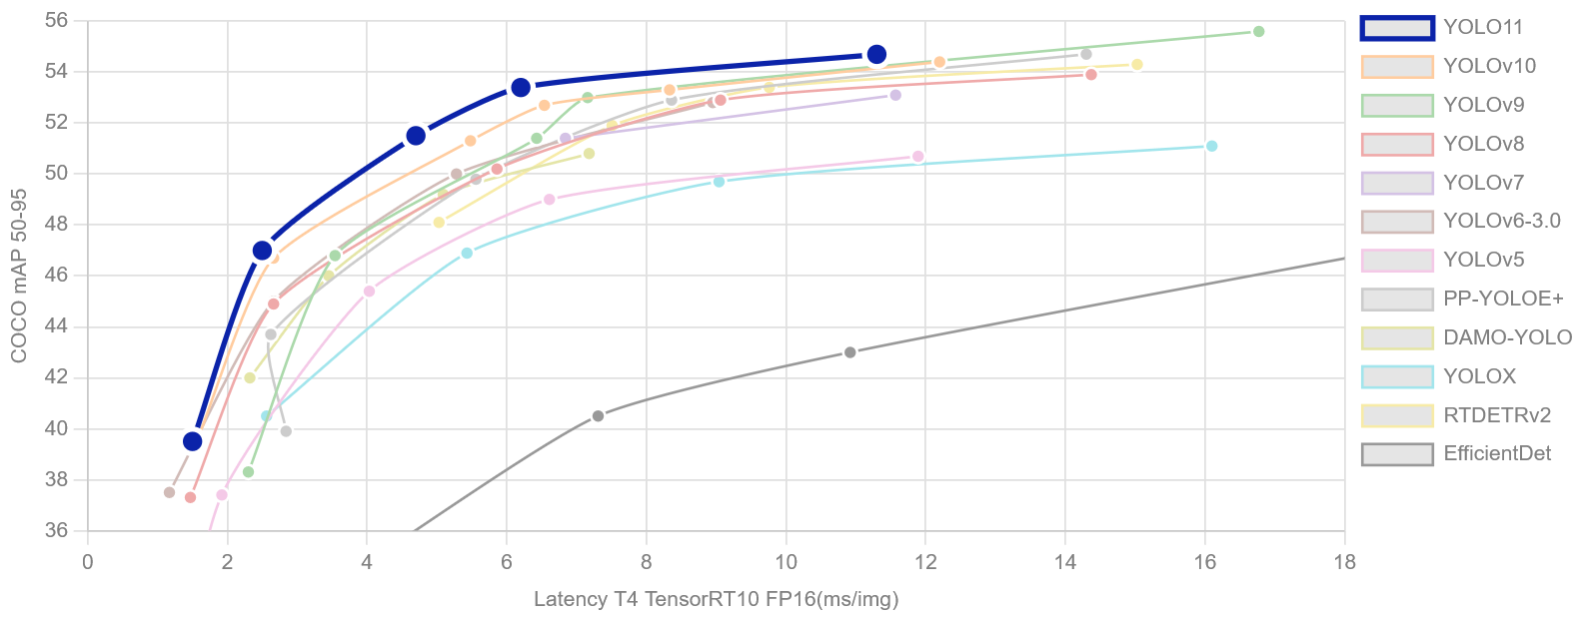
\includegraphics[width=1\textwidth]{figures/chapter03/YOLO11在COCO上的性能对比.png}
  \caption{YOLO11与其他主流网络在COCO数据集的性能对比\cite{jocherUltralyticsYOLO112024}}
  \label{YOLO11与其他主流网络在COCO数据集的性能对比}
\end{figure}

在YOLOv11系列的不同规模模型中，YOLO11n（nano版本）在精度与推理时间之间取得了较优折中。根据Ultralytics官方在COCO数据集上的检测模型指标\cite{jocherUltralyticsYOLO112024}，在输入尺寸为$640\times640$时，YOLO11n的mAP@0.5:0.95为$39.5\%$，参数量为$2.6\,\mathrm{M}$，计算量为$6.5\,\mathrm{B}$ FLOPs；其在CPU ONNX平台上的推理延迟为$56.1\pm0.8\,\mathrm{ms}$，在NVIDIA T4 TensorRT10平台上的推理延迟为$1.5\pm0.0\,\mathrm{ms}$。因此，综合检测精度、模型规模、推理延迟与工程可部署性，最终选定YOLO11n作为本系统的目标检测模型。

YOLO11n的整体结构如图\ref{YOLO11n整体结构}所示，主要包括以下三个部分：1、Backbone（主干网络）用于提取输入图像的多尺度特征表示。通过轻量化卷积模块与跨层连接结构，提高特征表达能力的同时控制参数规模和计算复杂度；2、Neck（特征融合网络）采用改进的特征金字塔结构（FPN/PAN类结构），实现不同尺度特征之间的自顶向下与自底向上融合，增强对小目标与远距离目标的检测能力；3、Head（检测头）负责输出边界框回归参数、目标置信度及类别概率。检测头通常采用解耦设计，将分类分支与回归分支分离，以提高收敛稳定性与定位精度。

在本系统中，YOLO11n输出的二维边界框信息将作为后续深度ROI提取与目标距离估计的空间约束基础。通过与双目立体匹配得到的深度图进行融合，系统能够完成目标检测、候选区域筛选和距离估计，从而为微型移动载具提供稳定、可部署的障碍物检测与测距能力。

\begin{figure}[h]
  \centering
  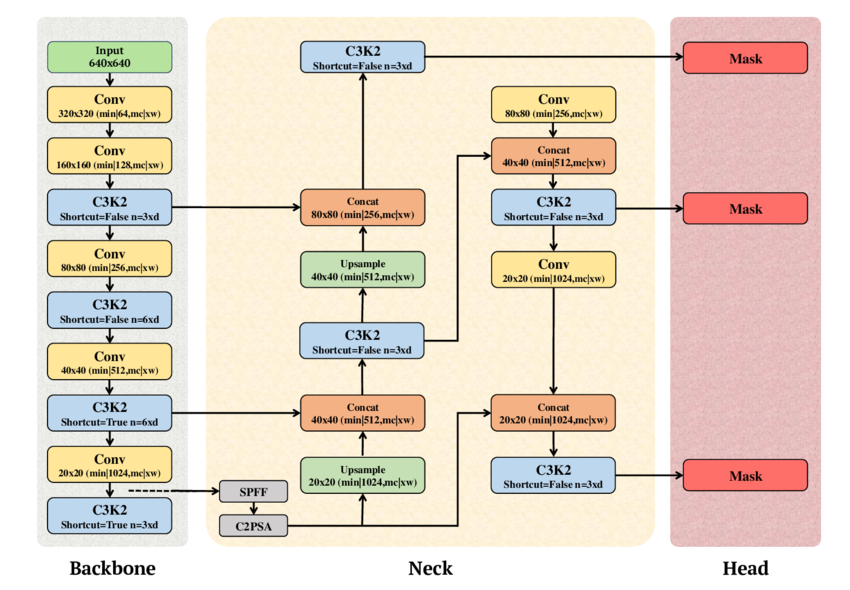
\includegraphics[width=1\textwidth]{figures/chapter03/YOLO11n整体结构.png}
  \caption{YOLO11n整体结构\cite{jocherUltralyticsYOLO112024}}
  \label{YOLO11n整体结构}
\end{figure}

\subsection{目标检测模型的训练}

本文采用“预训练+微调”的方式完成目标检测模型训练。具体而言，首先采用在COCO数据集上预训练的YOLO11n权重作为模型初始化参数，在此基础上再结合本文应用场景数据进行进一步微调，以提高模型对实际障碍物目标的识别能力。

COCO数据集是目标检测领域广泛采用的通用数据集，包含丰富的日常场景目标类别，可为模型提供较好的基础视觉特征表达能力\cite{linMicrosoftCOCOCommon2014}。通过引入COCO预训练权重，模型能够先学习常见目标的纹理、轮廓与语义信息，为后续面向具体场景的训练提供较好的参数初始化。

在完成预训练权重初始化后，本文采用VIDVIP数据集进行进一步微调\cite{babaVidvipDatasetObject2021b}。VIDVIP数据集面向人行道通行过程中的目标检测任务，包含行人、车辆、路侧障碍物等与移动平台通行安全密切相关的目标类别，其场景特征与本文面向园区道路环境的障碍物检测需求具有较高一致性。

目标检测模型的训练环境与第~\ref{sec:ch3-stereo-training-metrics}~节一致。经上述训练后，YOLO11n模型能够满足本文园区道路环境下对行人、车辆及路侧障碍物等目标的检测需求。

\section{基于双目视觉的目标空间定位算法研究}

在获得障碍物的二维检测结果后，需要进一步结合双目视觉深度信息，实现对目标空间距离及三维位置的估计。本文的障碍物测距算法以第~\ref{sec:ch3-object-detection}~节输出的目标检测结果为输入，融合立体匹配与双目成像几何模型，完成从图像平面到相机坐标系的空间恢复。整体测距流程如图\ref{目标检测及测距流程}所示，主要包括立体匹配与视差估计、视差到深度转换、目标区域深度估计以及目标三维坐标计算四个步骤。

\begin{figure}[h]
  \centering
  \includesvg[width=0.88\textwidth]{figures/chapter03/目标检测与测距流程}
  \caption{目标检测及测距流程}
  \label{目标检测及测距流程}
\end{figure}

（1）立体匹配与视差估计

对经过校正后的左右图像，采用前文提出的HAGVNet立体匹配模型进行视差估计，获得稠密视差图，如式~\eqref{eq:ch3-disparity}所示：
\begin{equation}\label{eq:ch3-disparity}
D=F(I_l,I_r)
\end{equation}
\begin{tabularx}{\textwidth}{@{}l@{\quad}r@{———}X@{}}
式中& $D$ & 视差图；\\
& $F(\cdot)$ & 立体匹配网络；\\
& $I_l,\,I_r$ & 校正后的左右图像。\\
\end{tabularx}\vspace{3.15bp}

根据双目成像原理，视差大小与目标距离呈反比关系，即视差值越大表示目标距离相机越近，视差值越小则对应较远的空间位置。

（2）深度恢复

根据双目成像几何模型，在相机完成标定且已知基线长度与焦距的条件下，可由视差图直接恢复稠密深度图$Z$，其关系如式~\eqref{eq:ch3-depth}所示：

\begin{equation}\label{eq:ch3-depth}
Z=\frac{fB}{D}
\end{equation}

（3）深度获取

由第~\ref{sec:ch3-object-detection}~节目标检测模块可获得每个障碍物在图像中的二维边界框。考虑到边界区域可能受到背景干扰、遮挡或视差不稳定等因素影响，本文对原始检测框进行等比例缩放，以目标中心为基准构造有效感兴趣区域（Region of Interest, ROI），如式~\eqref{eq:ch3-roi-scale}所示：
\begin{equation}\label{eq:ch3-roi-scale}
b_i'=\alpha b_i,\quad 0<\alpha<1
\end{equation}
\begin{tabularx}{\textwidth}{@{}l@{\quad}r@{———}X@{}}
式中& $b_i$ & 第$i$个目标的原始二维边界框；\\
& $b_i'$ & 缩放后的有效ROI；\\
& $\alpha$ & ROI缩放系数。\\
\end{tabularx}\vspace{3.15bp}

为降低异常深度值对测距结果的影响，本文在目标ROI内提取深度值，并采用其中位数作为目标的距离估计值，如式~\eqref{eq:ch3-depth-median}所示：
\begin{equation}\label{eq:ch3-depth-median}
\hat{Z}_i=\mathrm{median}\{Z(u,v)\mid (u,v)\in b_i'\}
\end{equation}
\begin{tabularx}{\textwidth}{@{}l@{\quad}r@{———}X@{}}
式中& $\hat{Z}_i$ & 第$i$个目标的深度估计值；\\
& $Z(u,v)$ & 深度图在像素$(u,v)$处的深度值；\\
& $(u,v)$ & 有效ROI内的像素坐标。\\
\end{tabularx}\vspace{3.15bp}

（4）目标三维坐标计算

在获得目标深度估计值后，可进一步恢复目标在相机坐标系下的三维空间位置。设目标中心在图像坐标系下的像素坐标为$(u_i,v_i)$，结合像素坐标到相机坐标系的转换模型，其三维坐标如式~\eqref{eq:ch3-xyz}所示：
\begin{equation}\label{eq:ch3-xyz}
X_i=\frac{(u_i-c_x)\hat{Z}_i}{f},\quad
Y_i=\frac{(v_i-c_y)\hat{Z}_i}{f},\quad
Z_i=\hat{Z}_i
\end{equation}
\begin{tabularx}{\textwidth}{@{}l@{\quad}r@{———}X@{}}
式中& $X_i,Y_i,Z_i$ & 第$i$个目标在相机坐标系下的三维坐标；\\
& $(u_i,v_i)$ & 第$i$个目标中心的像素坐标；\\
& $(c_x,c_y)$ & 相机主点坐标。\\
\end{tabularx}\vspace{3.15bp}

综合目标检测与深度估计结果，最终输出的障碍物信息如式~\eqref{eq:ch3-output}所示：
\begin{equation}\label{eq:ch3-output}
O_i=(c_i,s_i,X_i,Y_i,Z_i)
\end{equation}
\begin{tabularx}{\textwidth}{@{}l@{\quad}r@{———}X@{}}
式中& $O_i$ & 第$i$个障碍物的输出信息；\\
& $c_i$ & 目标类别；\\
& $s_i$ & 检测置信度。\\
\end{tabularx}\vspace{3.15bp}

目标检测与定位结果如图\ref{障碍物检测与定位效果图}所示。图中上方为左视图，中间为深度图，其中颜色由蓝到红表示目标距离由近到远；下方为检测结果，检测框标示出识别到的目标，标签中给出了类别、置信度及其坐标信息。

\begin{figure}[h]
  \centering
  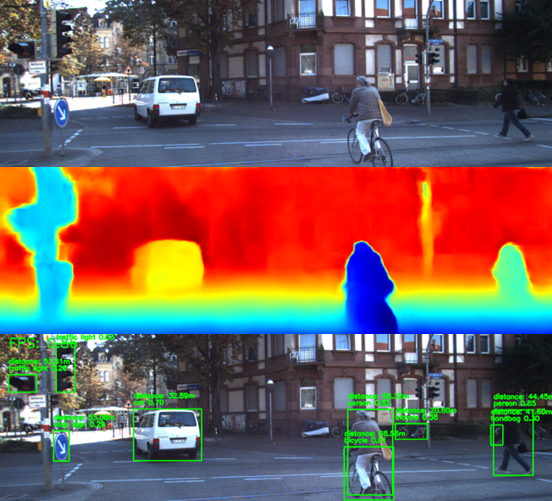
\includegraphics[width=0.7\textwidth]{figures/chapter03/障碍物检测与定位结果.png}
  \caption{障碍物检测与定位效果图}
  \label{障碍物检测与定位效果图}
\end{figure}
\FloatBarrier

\section{本章小节}

本章围绕双目视觉环境感知需求，完成了双目标定与校正、立体匹配、目标检测与空间定位算法的设计与验证。在双目测距基础部分，基于双目成像几何模型与相机标定方法，完成了双目标定与校正，为后续视差估计与深度计算提供了可靠的几何基础。在立体匹配方面，提出轻量化模型 HAGVNet。该模型通过分层注意力引导代价体构建机制，在较低计算量下提升匹配稳定性与精度，满足嵌入式平台实时测距需求。在目标检测方面，采用轻量化一阶段模型 YOLO11n，实现典型障碍物的快速识别与边界框输出。结合检测结果与深度信息，构建目标级空间定位方法，实现由二维检测到三维距离估计的转换。本章完成了双目视觉感知算法体系的构建，为整车系统集成与实验验证提供了算法基础。
